\newpage
\pdfbookmark[1]{Visuaalne kokkuvõte}{visualsummary}
\section*{Visuaalne kokkuvõte}

\begin{center}
    % Kasutame 'height', et pilt mahuks pealkirja alla. 
    % 0.7\textheight jätab piisavalt ruumi pealkirjale ja marginaalidele.
    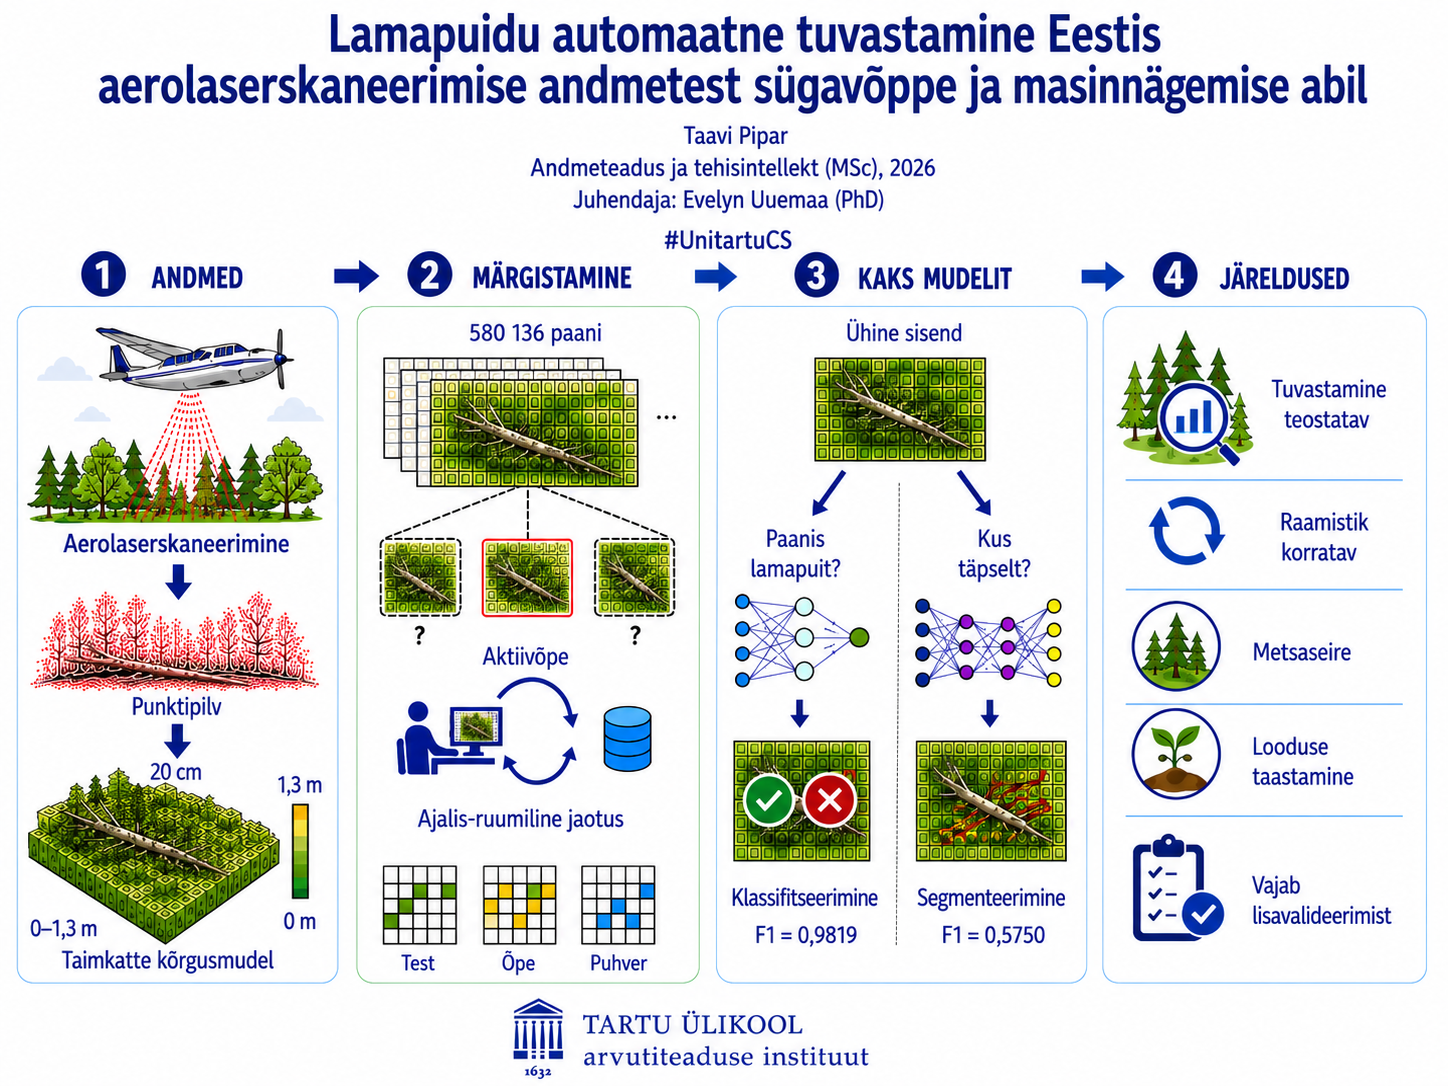
\includegraphics[height=0.65\textheight, angle=90, keepaspectratio]{estonian/joonised/Lamapuit_est.png}
    
    \stepcounter{figure} % Suurendame käsitsi jooniste loendurit
    \small JOONIS \thefigure: Visuaalne kokkuvõte % Kui soovid joonise allkirja
    \label{fig:visuaalne-kokkuvõte}
\end{center}

\newpage
\pdfbookmark[1]{Visual abstract}{visualabstract-en}
\section*{Visual abstract}

\begin{center}
    % Kasutame sama paigutust nagu eestikeelse visuaalse kokkuvõtte puhul.
    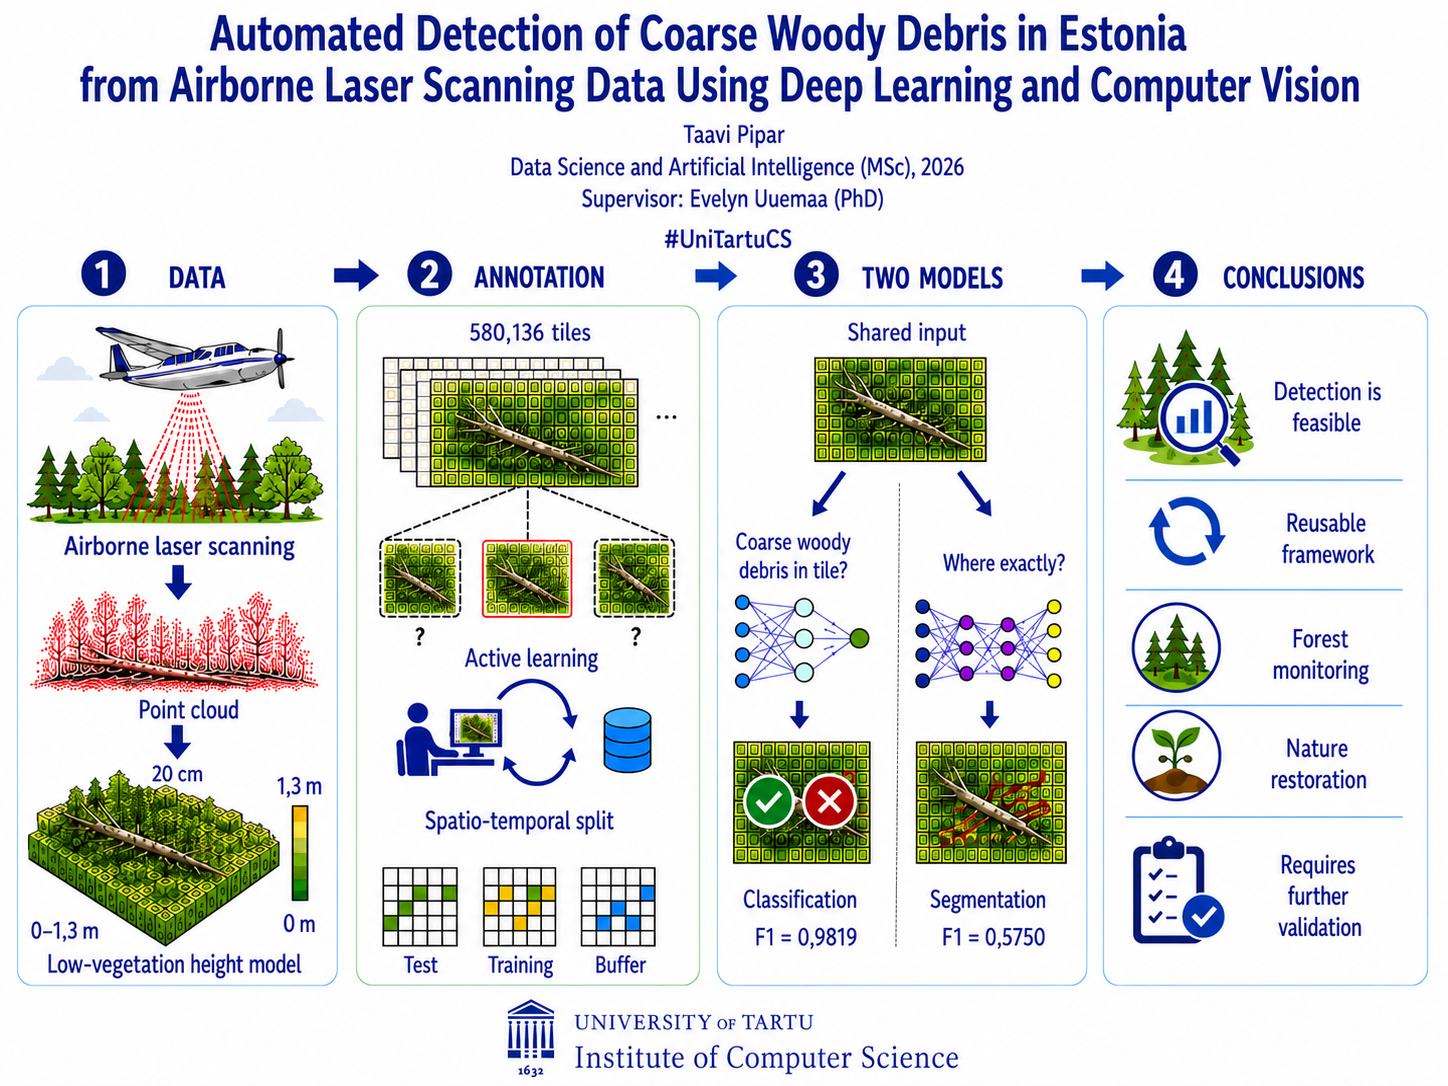
\includegraphics[height=0.65\textheight, angle=90, keepaspectratio]{estonian/joonised/Lamapuit_eng.png}
    
    \stepcounter{figure}
    \small FIGURE \thefigure: Visual abstract
    \label{fig:visual-abstract}
\end{center}

\newpage
